\documentclass{article}

\usepackage[a4paper,left=1in,right=1in,showframe]{geometry}
\usepackage{tikz}

%% \printhex[number of digits]{decimal value}
%% number of digits between 1 and 8
%% decimal value: TeX counter value
%% \hexdiv = divider, power of 16
%% \hexvar = number to be converted
%% \hextmp = scratch calculation counter
\newcount\hexdiv
\newcount\hexvar
\newcount\hextmp
\newcommand{\printhex}[2][4]{%
%\hexdiv=0\hexvar=0\hextmp=0
\hextmp=#1%
\ifnum#1>7
\hextmp=#2
\ifnum\hextmp<0\relax
\advance\hextmp by 2147483647\advance\hexvar by 1
\divide\hextmp by 268435456
\advance\hextmp by 8
\printhexdigit\hextmp\relax
\else
\divide\hextmp by 268435456
\printhexdigit\hextmp\relax
\fi
\fi
\hexvar=#2%
\hexdiv=0\ifcase#1\relax \or 16\or 256\or 4096\or 65536\or 1048576\or 16777216\or 268435456\else 268435456\fi
\ifnum\hexvar<0\relax\advance\hexvar by 2147483647\advance\hexvar by 1\fi
\hextmp=\hexvar
\divide\hextmp by \hexdiv%
\multiply\hextmp by \hexdiv
\advance\hexvar by -\hextmp
\divide\hexdiv by 16%
\loop
	\hextmp=\hexvar
	\divide\hextmp by \hexdiv
	\printhexdigit\hextmp\relax
	\multiply\hextmp by \hexdiv
	\advance\hexvar by -\hextmp
	\divide\hexdiv by 16
	\ifnum\hexdiv>0
\repeat
}
\newcommand{\printhexdigit}[1]{%
	\ifcase#1\relax 0\or 1\or 2\or 3\or 4\or 5\or 6\or 7\or 8\or 9\or A\or B\or C\or D\or E\or F\else ***error***\fi
}

% Define our lightning symbol in Tikz
\def\Lightning{\tikz\draw (0,0) -- ++(0.40,0.10) -- ++(-0.25,0) -- ++(0.40,0.10);}

%% This command draws a populated stack from bottom to top and leaves one
%% memory location unpopulated and points the stack pointer to it
%% Call by: \drawstack[address_bottom_of_stack]{tikz node position}{stack contents}
%% Example: \drawstack[0x85f]{0,0}{pcl,pch,0xff,0x55,R16,R16}
\newcounter{stackaddress}
\newcommand{\drawstack}[3][-1]{%
\setcounter{stackaddress}{#1}%
\node at (#2) (startpoint) {};
\draw (startpoint) ++(1.5,0)
   \foreach \label in {#3} {
      ++(-1.5,0) rectangle node {\label} ++(1.5,0.5) node[pos=0.5,right,xshift=0.8cm] {\ifnum\thestackaddress>-1\relax 0x\printhex[3]{\thestackaddress}\fi}
	  \pgfextra{\addtocounter{stackaddress}{-1}}
   }
   ++(-1.5,0) rectangle node {} ++(1.5,0.5) node[pos=0.5,right,xshift=0.8cm] {\ifnum\thestackaddress>-1\relax 0x\printhex[3]{\thestackaddress}\fi}
   ++(0,0) -- ++(0,1)
   ++(-1.5,0) -- ++(0,-1)
   ++(0,-0.25) node[left,xshift=2pt] {sp \tikz[thick,baseline=-0.5ex,->] \draw (0,0) -- ++(0.6,0);}
;
}


% Style for picturing interrupt routines and subroutines
\tikzset{bookirqsub/.style={line width=1pt,font=\sffamily,-latex}}

\usepackage{show2e}
\showcmd\printhex
\showcmd\drawstack

\begin{document}

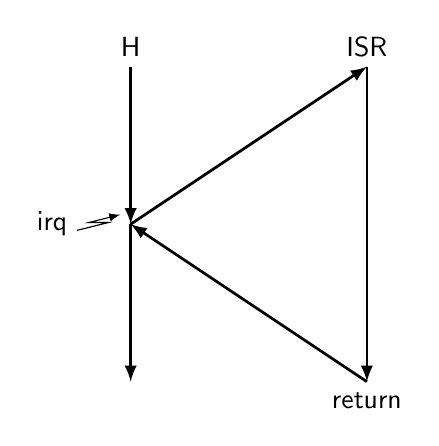
\begin{tikzpicture}[bookirqsub]
\draw (0,0)  node (H) [above] {H}  -- (0,-2) node (irq) [left] {irq \Lightning};
\draw (0,-2) -- (3,0) node[above] {ISR};
\draw (3,0)  -- (3,-4) node[below] {return};
\draw (3,-4) -- (0,-2);
\draw (0,-2) -- (0,-4);
\end{tikzpicture}

\vspace*{1cm}

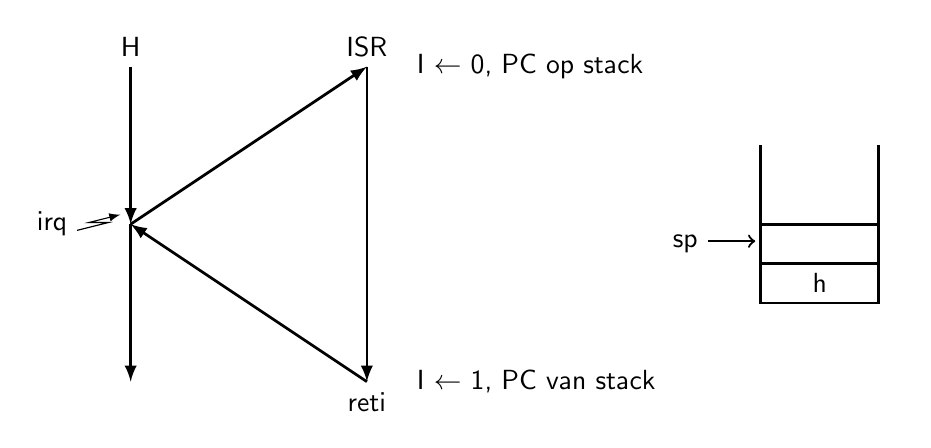
\begin{tikzpicture}[bookirqsub]
\draw (0,0)  node (H) [above] {H}  -- (0,-2) node (irq) [left] {irq \Lightning};
\draw (0,-2) -- (3,0) node[above] {ISR} node [right, xshift=.5cm] {I $\leftarrow$ 0, PC op stack};
\draw (3,0)  -- (3,-4) node[below] {reti} node [right, xshift=.5cm] {I $\leftarrow$ 1, PC van stack};
\draw (3,-4) -- (0,-2);
\draw (0,-2) -- (0,-4);
\drawstack{8,-3}{h}
\end{tikzpicture}

\vspace*{1cm}

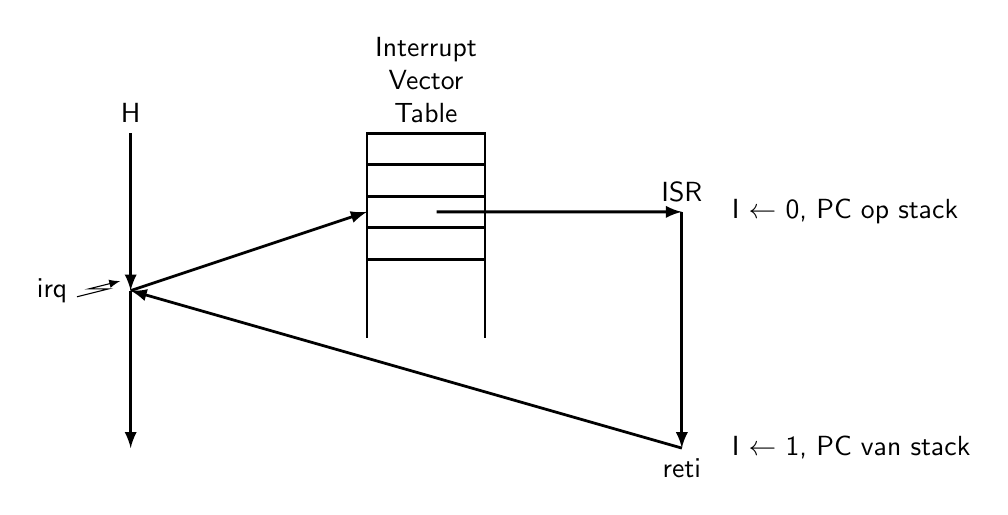
\begin{tikzpicture}[bookirqsub]
\draw (0,0)  node (H) [above] {H}  -- (0,-2) node (irq) [left] {irq \Lightning};
\draw (3,0) rectangle ++(1.5,-0.4) node[above,pos=0.5,yshift=2mm,align=center] {Interrupt\\Vector\\Table}
            rectangle ++(-1.5,-0.4)
            rectangle ++(1.5,-0.4) node[pos=0.5] (A) {}
			rectangle ++(-1.5,-0.4)
               --     ++(0,-1)
  ++(1.5,1)    --     ++(0,-1);
\draw (0,-2) -- (3,-1);
\draw (0,-2) -- (0,-4);
\draw (A) -- (7,-1) node [above] {ISR} node [right, xshift=.5cm] {I $\leftarrow$ 0, PC op stack};
\draw (7,-1) -- (7,-4) node[below] {reti} node [right, xshift=.5cm] {I $\leftarrow$ 1, PC van stack};
\draw (7,-4) -- (0,-2);
\end{tikzpicture}

%%
%% Stack
%%

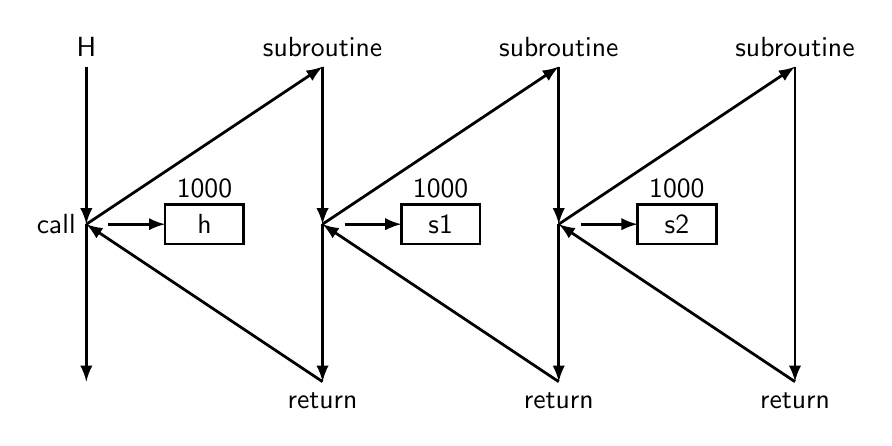
\begin{tikzpicture}[bookirqsub]
\draw (0,0)  node (H) [above] {H}  -- (0,-2) node (call) [left] {call};
\draw (0,-2) -- (3,0) node[above] {subroutine};
\draw (3,0)  -- (3,-2);
\draw (3,-2) -- (3,-4) node[below] {return};
\draw (3,-4) -- (0,-2);
\draw (0,-2) -- (0,-4);
\draw (0+8pt,-2) -- (1,-2);
\draw[-] (1,-2.25) rectangle ++(1,0.5) node[pos=0.5] {h} node[pos=0.5,yshift=0.45cm] {1000};
\draw (3,-2) -- (6,0) node[above] {subroutine};
\draw (6,0)  -- (6,-2);
\draw (6,-2) -- (6,-4) node[below] {return};
\draw (6,-4) -- (3,-2);
\draw (3cm+8pt,-2) -- (4,-2);
\draw[-] (4,-2.25) rectangle ++(1,0.5) node[pos=0.5] {s1} node[pos=0.5,yshift=0.45cm] {1000};
\draw (6,-2) -- (9,0) node[above] {subroutine};
\draw (9,0)  -- (9,-4) node[below] {return};
\draw (9,-4) -- (6,-2);
\draw (6cm+8pt,-2) -- (7,-2);
\draw[-] (7,-2.25) rectangle ++(1,0.5) node[pos=0.5] {s2} node[pos=0.5,yshift=0.45cm] {1000};
\end{tikzpicture}

\vspace*{1cm}

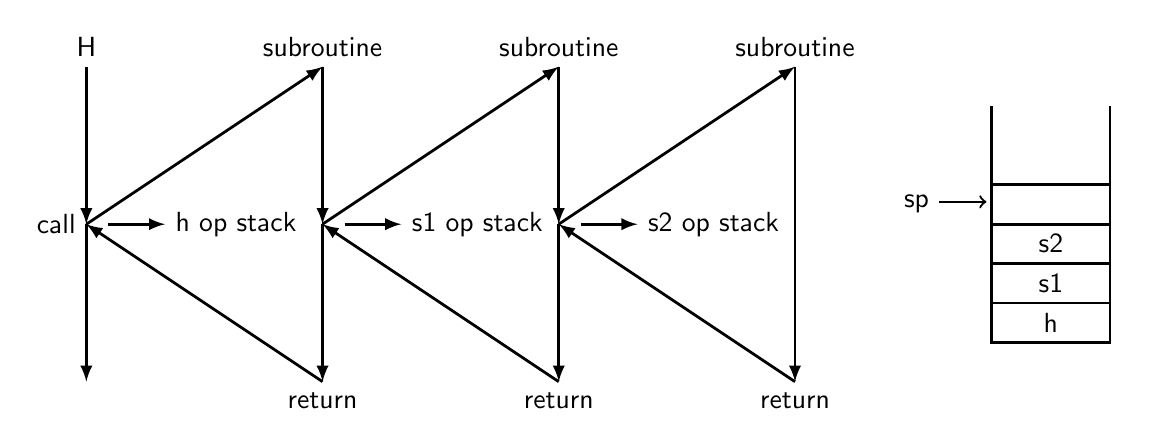
\begin{tikzpicture}[bookirqsub]
\draw (0,0)  node (H) [above] {H}  -- (0,-2) node (call) [left] {call};
\draw (0,-2) -- (3,0) node[above] {subroutine};
\draw (3,0)  -- (3,-2);
\draw (3,-2) -- (3,-4) node[below] {return};
\draw (3,-4) -- (0,-2);
\draw (0,-2) -- (0,-4);
\draw (0+8pt,-2) -- (1,-2);
\node at (1,-2) [right] {h op stack};
\draw (3,-2) -- (6,0) node[above] {subroutine};
\draw (6,0)  -- (6,-2);
\draw (6,-2) -- (6,-4) node[below] {return};
\draw (6,-4) -- (3,-2);
\draw (3cm+8pt,-2) -- (4,-2);
\node at (4,-2) [right] {s1 op stack};
\draw (6,-2) -- (9,0) node[above] {subroutine};
\draw (9,0)  -- (9,-4) node[below] {return};
\draw (9,-4) -- (6,-2);
\draw (6cm+8pt,-2) -- (7,-2);
\node at (7,-2) [right] {s2 op stack};
\drawstack{11.5,-3.5}{h,s1,s2}
\end{tikzpicture}

\vspace*{1cm}

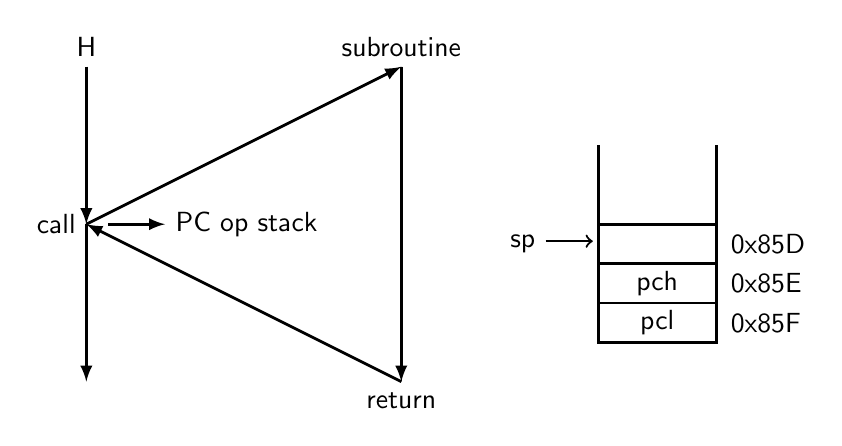
\begin{tikzpicture}[bookirqsub]
\draw (0,0)  node (H) [above] {H}  -- (0,-2) node (call) [left] {call};
\draw (0,-2) -- (4,0) node[above] {subroutine};
\draw (4,0)  -- (4,-4) node[below] {return};
\draw (4,-4) -- (0,-2);
\draw (0,-2) -- (0,-4);
\draw (0+8pt,-2) -- (1,-2);
\node at (1,-2) [right] {PC op stack};
\drawstack[2143]{6.5,-3.5}{pcl,pch}
\end{tikzpicture}

\noindent\hrulefill

0x\printhex[8]{-1} 0x\printhex[8]{2124000000}

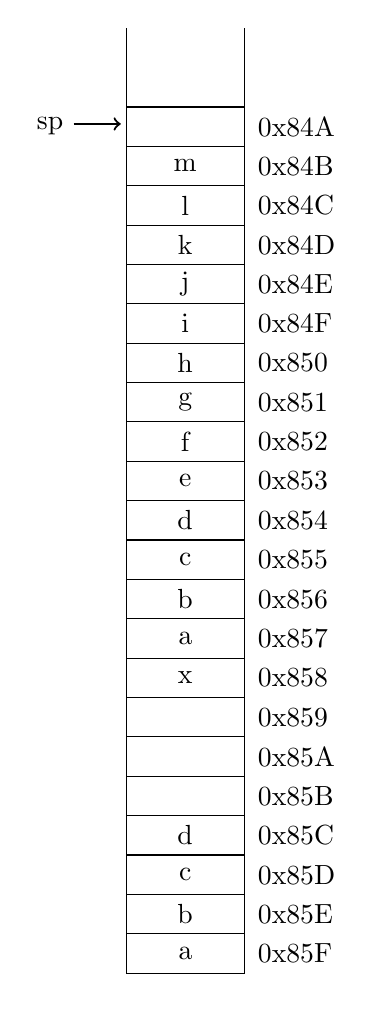
\begin{tikzpicture}
\drawstack[2143]{0,0}{a,b,c,d,,,,x,a,b,c,d,e,f,g,h,i,j,k,l,m};
\end{tikzpicture}

\end{document}